\chapter{Softwares Para Bibliotecas Digitais}
\label{Att:anexobibliotecas}

Nesse anexo estão apresentados os principais produtos de software relacionados a bibliotecas digitais que foram investigados durante o período de preparação do Trabalho de Conclusão de Curso 1.

\section*{Greenstone} 
Greenstone\footnote{Disponível em \url{http://www.greenstone.org}.} é um conjunto de softwares para a construção e distribuição de coleções de bibliotecas digitais. Ele organiza a informação, publicando-a na Internet ou em CD-ROM. Greenstone é produzido pela Universidade de Waikato, desenvolvido e distribuído em cooperação com a UNESCO e a ONG Human Info.

Possui suporte para multiplas plataformas sendo elas: Unix, Windows e Mac OSX. Ele é distribuído sobre licença GNU GPL v3. Também possui suporte para multilinguagem, que são ajustadas em suas configurações. Compatível com a especificação para o conjunto de metadados DublinCore e também é possível a utilização do protocolo OAI-PMH.

O objetivo do software Greenstone é capacitar os usuários, especialmente em universidades, bibliotecas e outras instituições de serviço público, para construir suas próprias bibliotecas digitais. Através de plugins, Greenstone pode importar documentos digitais em formatos de texto incluindo HTML, JPG, TIFF, MP3, PDF, vídeo e Word. Textos, PDF, HTML e documentos similares são convertidos em Greenstone Archive Format (GAF), que é um formato XML equivalente. Caso o arquivo não seja disponibilizado na lista padrão que o GreenStone fornece, pode ser desenvolvido um plug-in para manuseio do formato do arquivo em questão.

O GreenStone possui a vantagem de ser altamente customizável, tanto no quesito de disponibilização de uma inteface web compatível com o desejo do administrador, quanto na disponibilização de itens de acordo com o especificado na ferramenta de criação de uma bilioteca digital. Esse software é capaz de exportar os dados que compõe a bilioteca (textos, XML, entre outros) para uma mídia de CD/DVD-ROM, ou mesmo, exportado para um arquivo que pode ser utilizado para ser importado novamente em outro ambiente que possua o GreenStone.

Para disponibilização e criação de bibliotecas utilizando o GreenStone, existem 3 métodos de criação, descritos a seguir:

\begin{itemize}
  \item \textbf{GLI} (GreenStone Library Interface) É composto por um programa escrito em java, isso faz com que o GLI consiga rodar em qualquer sistema operacional.  A partir de versão 2.4 do GreenStone, o GLI tomou força entre os usuários e tassou a ser o padrão para a criação de bibliotecas digitais, principalmente por ter facilitado a criação de bibliotecas digitais, pois a sua interface é de fácil complexidade e muito boa usabilidade. Contém um conjunto de metadados já definido, além de ser possível criar as próprias;
  \item \textbf{Terminal} (Uso de linhas de Comando) Através de comandos na linhas de comando é possível criar uma biblioteca. Esses comandos chamam uma biblioteca escrita na linguagem Perl, que monta as bibliotecas de acordo com os comandos utilizados; e
  \item \textbf{Interface Web} Também pode-se criar uma biblioteca através da interface web, através do painel de administração citado anteriormente.
\end{itemize}

Independentemente desses três modos de criação de uma biblioteca digital, existem três passos para a criação de uma biblioteca digital, eles são: Obter, Enriquecer, Design e Criar.

Na etapa "Obter" são coletados os dados que vão alimentar a biblioteca digital, eles podem ser em vários formatos (destacados anteriormente), ou mesmo, um download de vários arquivos do site utilizando wget. É onde os arquivos vão ser colocados. Na etapa "Enriquecer" são inseridos metadados para as mídias digitais que foram obtidas anteriormente. Na etapa "Design" há a customização da sua biblioteca digital, nessa etapa há a criação da estrutura para pesquisa mais elaboradas, macros, pesquisa nas páginas, estrutura dentro dos documentos, customização das páginas, categorização da informação, entre outros. Por fim, na etapa "Criar", constrói toda a biblioteca digital. Esse passo leva um tempo, pois ele vai compilar todas as informações que foram definidas nos passos anteriores. Caso seja de interesse do usuário é possível o usuário dar um preview da informação antes da criação da biblioteca digital.

Os plugins são utilizados para visualização de documentos e extração de metadados de um determinado tipo de arquivo. Cada tipo de arquivo tem um plugin específico que pode ser utilizado para abrir o mesmo no greenstone, assim como preencher os metadados automaticamentes na parte de enriquecer, basta somente que o usuário direcione o plugin para ler os metadados nos arquivos que foram obtidos. Por exemplo, alguns plug-ins juntamente com o arquivo que ele abre são: (i) BibTexPlugin – Extensão que manuseia arquivos com a extensão .bibtex; (ii) CSVPlugin – Extensão que manuseia arquivos com a extensão .csv separados por vírgulas, cada titulo pode ser definido como um metadado; e (iii) HTMLPlugin – Arquivos .HTML (hipertexto) são abertos com esse plugin. Através das meta tags especificadas pela W3C (meta name), podemos fazer o greenstone obter os registros de metadados diretamente dos arquivos. Vale ressaltar que existem muitas outras extensões que estão documentadas na wiki oficial do greenstone \footnote{Disponível em \url{http://wiki.greenstone.org/wiki/index.php/Plugins}.}.

Uma das vantagens do GreenStone é possível a utilização de metadados. Existem várias especificações de metadados definidas no GreenStone, entre eles, o DublinCore, o DLS e o EX, esse último vem automaticamente sobre o arquivo como nome, tamanho, data de criação, entre outros, quando o dado é importado para dentro da biblioteca digital. Esses dados geralmente são preenchidos automaticamente e não são editáveis. Também podemos utilizar os plugins para preenchimentos desses metadados, basta apenas apontar para o local onde esses metadados estão especificados (tags XML, meta name, título de um campo CSV, entre outros.). Após a configuração, basta o usuário passar para a fase de criação, onde o GreenStone utiliza o plugin para análise do arquivo e extração dos metadados, que serão automaticamente exportados em formatos de metadados na aba de enriquecimento.

Existem mais metadados no GreenStone especificados por outras entidades, além de permitir a possibilidade do usuário criar os seus próprios metadados. Na seção 2, foi especificado para o Participa.Br um conjunto de metadados para os mecanismos formais de participação.

A interface principal para a visualização da biblioteca digital é disponibilizada através de uma interface web, desenvolvida na lingiagem Java. Não há restrição para a utilização da interface, visto que não tem recursos complexos de script e CSS. Para disponibilizar essa interface web, o GreenStone possui um servidor web que roda o servidor Apache Tomcat.

A medida em que foi definido na criação de conteúdo, o usuário pode acessar as mídias digitais de diversas formas, podemos citar por exemplo, a categorização da informação, onde o usuário acessa as mídias através de categorias. Podemos também definir o modelo da nossa barra superior, colocando itens relevantes para o acesso mais rápido. Dentro das mídias digitais, pode-se colocar somente itens relevantes e que sejam úteis para o usuário.

No GreenStone, também é possível ter uma interface web para a administração, onde é possível gerenciar as contas (criar, deletar, editar e obter), esconder bibliotecas (por exemplo, no caso da manutenção da mesma), segurança das mídias digitais através de criptografia com senha. Mais abaixo serão especifícado mais detalhes técnicos sobre a Interface do GreenStone.

Apesar de usar tags que são obsoletas e não usáveis , a customização no GreenStone é bastante flexível e permite a criação de temas com bastante agilidade e facilidade, isso se deve a modularização dos arquivos do tema, isto é, não existe somente um arquivo HTML ou um arquivo de configuração para a personalização do tema. Tanto no GreenStone 2 ou em sua versão mais recente, os arquivos de estilo estão em pasta separadas dos arquivos de macro, assim como as imagens que o GreenStone carrega, isso  facilita personalização da página pelo desenvolvedor. Através de pesquisas é possível acessar diversos tutorias que ensinam a personalizar o tema.

No GreenStone 2, existem seis lugares essenciais para a personalizar a página, mudando o estilo nos arquivos CSS ou colocando/removendo imagens conforme a Figura \ref{fig:esqueletogreenstone}.

\graphicspath{{figuras/}}
\begin{figure}[H]
\centering
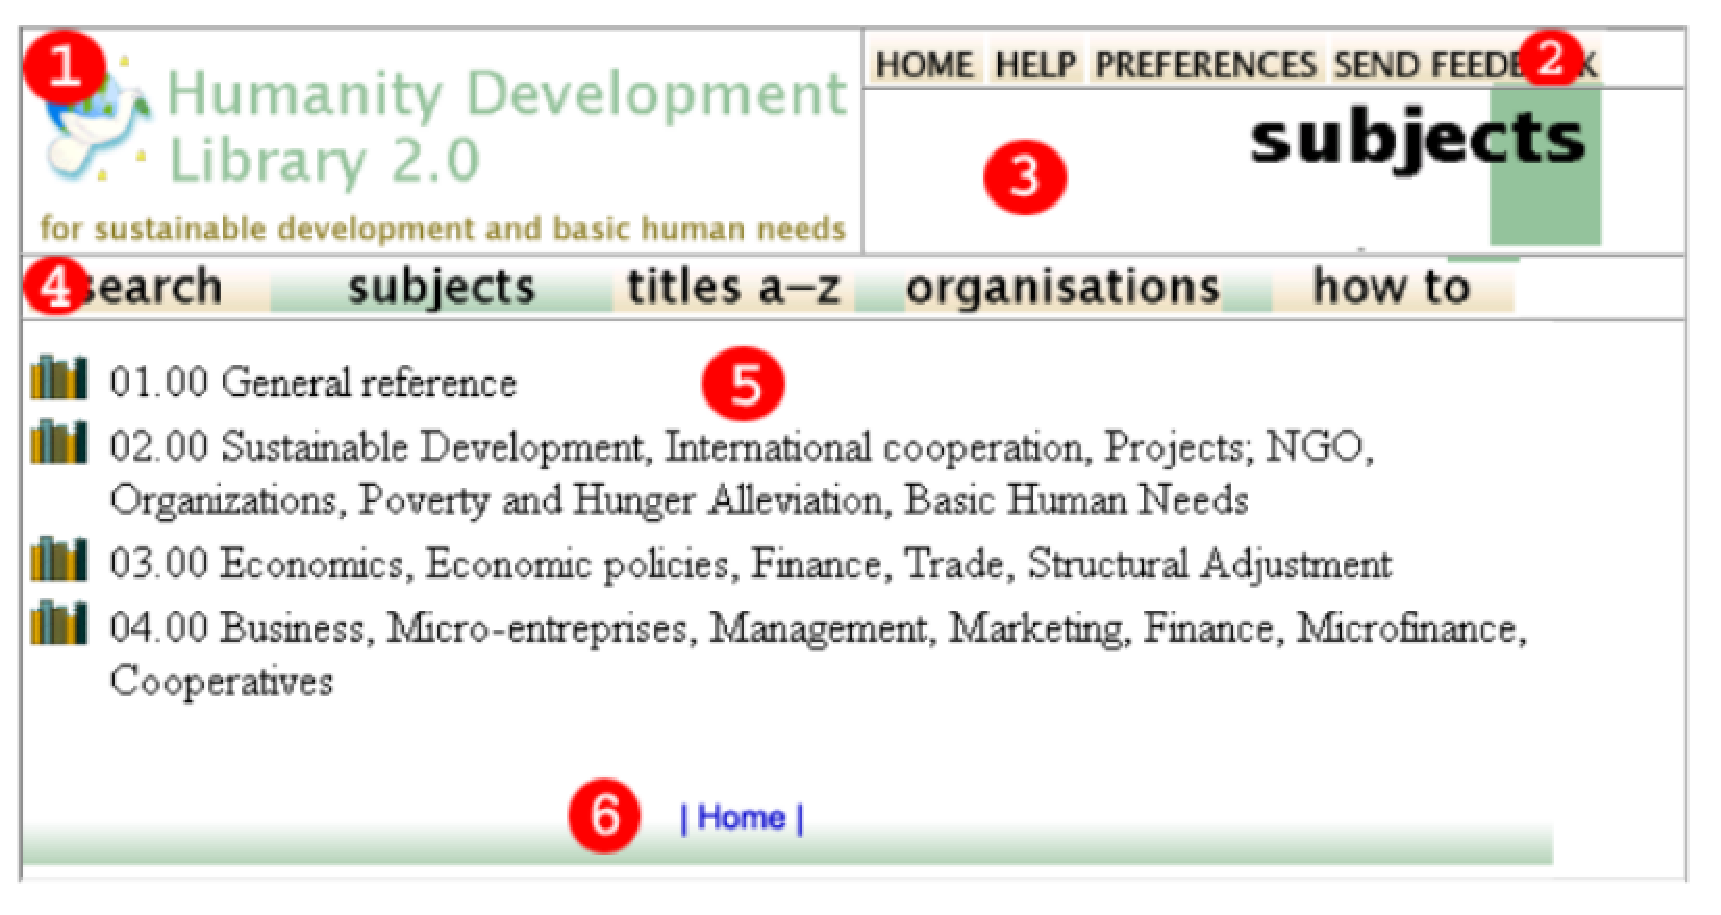
\includegraphics[width=0.5\textwidth]{esqueleto_greenstone}
\caption{Personalização do GreenStone}
\label{fig:esqueletogreenstone}
\end{figure}
%Figura A.1: Personalização do GreenStone.

\begin{enumerate}
  \item \textbf{Logo} A logo é a imagem que vai ficar presente em todas as páginas. O usuário pode alterar a logo no GreenStone para uma imagem ou texto.
  \item \textbf{Barra superior} Nessa área, os usuários podem escolher funções de personalização da página, ajuda, acessar a home entre outros. Através da personalização. pode-se mudar a barra superior, escondendo ou mostrando funções.
  \item \textbf{Titulo da página} Titulo de cada seção da página. Assim como na logo, pode-se colocar imagens ou texto.
  \item \textbf{Barra superior} Na barra superior, mostra todas as opções que serão pesquisadas e navegadas. Utilizando o GLI, podemos escolher esses elementos que serão pesquisados (títulos, subtítulos, arquivos, etc.). Já nos arquivos, podemos editar o estilo do mesmo.
  \item \textbf{Área do Documento} Área de disponibilização do documento, onde ser pode pesquisar e obter todos os documentos da biblioteca digital.
  \item \textbf{Footer} O rodapé da página, que pode ser um link, texto ou imagens.
\end{enumerate}

Para a montagem do HTML, o GreenStone divide a sua interface em macros, que controlam a montagem de todas as páginas, isto é, cada macro é um pedaço de HTML ou mesmo texto puro e sua junção é toda a interface que o GreenStone carrega. Para identificar as macros no GreenStone, elas ficam dentro da pasta macros a partir do diretório raiz do GreenStone, eles possuem extensão .dm relacionado com a função que executam (exemplo: a página de sobre o GreenStone possui a macro about.dm). Dentro do arquivo, cada macro é definido por \_ (underline) tanto no início como no final (exemplo: \_matches\_).  A macro como funciona como uma extensão de uma função C++ dentro do GreenStone, ou seja, após especificarmos uma macro com \_ (underline), utiliza-se as {} (colchetes) para determinar o que aquela macro vai fazer e pode-se reutilizar essa macro em outros arquivos. No GreenStone 2, as imagens e arquivos de estilo ficam dentro de suas respectivas pastas, isso ajuda na organização do arquivo, que consequentemente, ajuda na manutenção e evolução do mesmo,

Existe ainda uma outra versão do Greenstone (Greenstone 3) que, diferentemente do GreenStone 2, a sua nova versão utiliza o JSP, onde a idéia de funcionamento é a mesma, cada função está relacionada dentro de um arquivo.
 
No GreenStone 3 em vez de macros, são utilizados templates xsd, onde o conjunto do mesmo forma a página HTML. Dentro de um template, podemos definir textos ou tags HTML e chamamos o mesmo dentro do local onde precisamos daquele template. Assim como no GreenStone 2, na versão 3, os arquivos são organizados separadamente, só que dessa vez, cada tema possui sua pasta de estilos, scripts e imagens, facilitando mais ainda na manutenção e criação de novos temas.

\section*{KEA}

No KEA\footnote{Maiores informações disponíveis em: \url{http://www.nzdl.org/Kea}.} palavras/frases-chave são amplamente utilizadas em grandes coleções de documentos. Elas descrevem o conteúdo dos documentos e fornecem uma espécie de metadados semânticos úteis para uma grande variedade de propósitos. A tarefa de atribuir frases-chave a um documento é chamada de indexação keyphrase. Por exemplo, trabalhos acadêmicos são frequentemente acompanhados por um conjunto de frases livremente escolhidas pelo autor. Em bibliotecas, indexadores profissionais selecionam frases-chave de um vocabulário controlado (também chamado Subject Headings) de acordo com regras da catalogação definida. Na Internet, bibliotecas digitais, ou qualquer outro depósito de dados também usam frases (tags ou etiquetas de conteúdo) para organizar e proporcionar um acesso temático aos seus dados.

KEA é um algoritmo para extração de frases a partir de documentos de texto. Ele pode ser usado para indexação livre ou para a indexação com um vocabulário controlado. Entre outras características, o KEA possui várias versões, é implementado em Java e é independente de plataforma. Além disso, é um software open-source distribuído sob a licença GNU.

\section*{Omeka}

Omeka\footnote{Disponível em \url{http://www.omeka.org}.} é uma plataforma para disponibilização e manutenção de  bibliotecas digitais bem flexível, isto é, ele se adapta muito bem para sua finalidade, seja ele múseu, biblioteca de imagens, livros, lugares (bibliotecas sobre guerras), entre outros. O Omeka é um software livre, com código aberto e escrito em PHP. Sua instalação é bastante simples, bastando apenas que a máquina do cliente possua o PHP 5 instalado, juntamente com o banco de dados MySQL e um servidor HTTP (como o apache ou nginx). O Omeka não possui uma finalidade específica como o GreenStone, Dspace, entre outros. Na figura \ref{fig:finalidadeomeka} podemos visualizar que o Omeka caminha na intersecção de três ferramentas, entre elas: Sistema de gerenciamento de conteúdo (Web Content Management ou CMS), Repositório de arquivos digitais e coleções (Livraria Digital) e Sistemas para gerenciamento de museus.

\graphicspath{{figuras/}}
\begin{figure}[H]
\centering
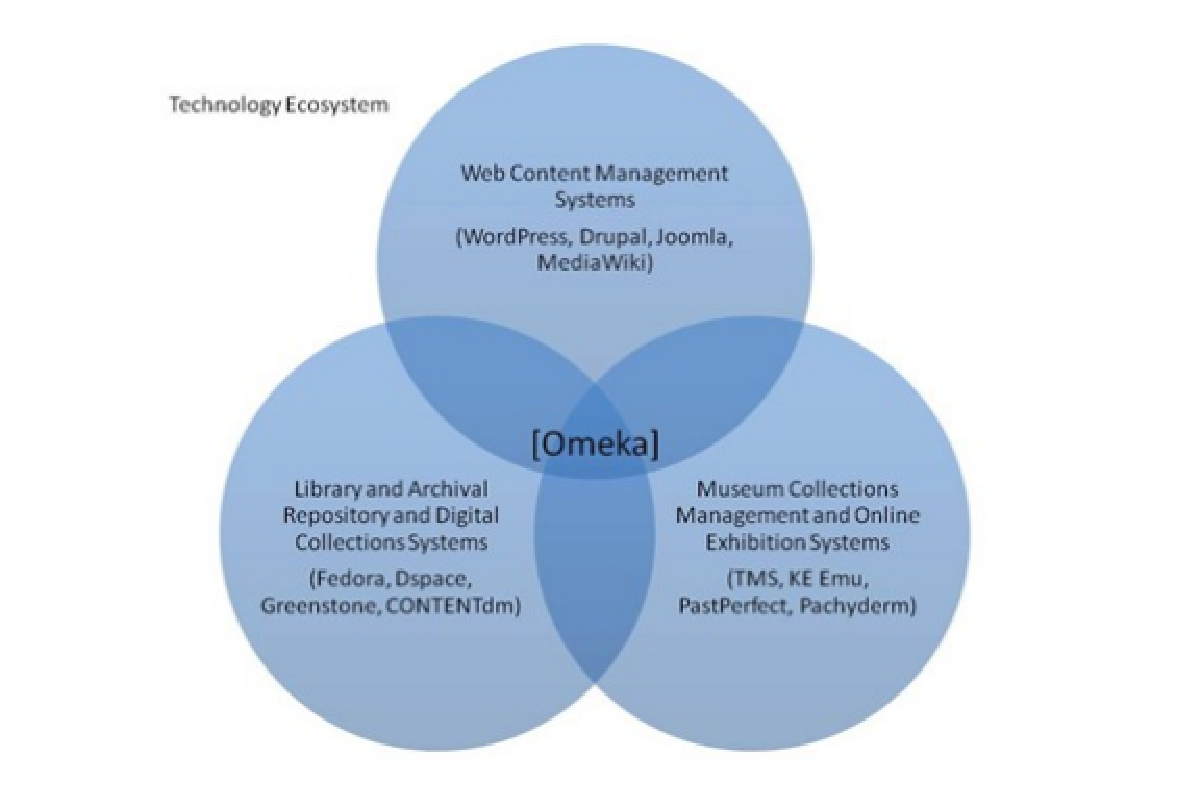
\includegraphics[width=0.7\textwidth]{finalidade_omeka}
\caption[Finalidade do Omeka]{Finalidade do Omeka. Retirado do Site \url{http://www.omeka.org}}
\label{fig:finalidadeomeka}
\end{figure}
%Figura A.2: Finalidade do Omeka Retirado de OMEKA.ORG

O Omeka possui uma interface muito intuítiva e de fácil personalização, isso se deve ao fato de ser construído para pessoas que não são experiêntes na utilização de computadores. Diferentemente do GreenStone, o Omeka não possui uma interface offline para inserção de dados, já que todas as funções são realizadas dentro do site. Sua arquitetura possui o padrão MVC (Model-View-Controller) que foi visto na seção \ref{sub:arquiteturamvc}.  

Outro padrão arquitetural que o Omeka possúi é sua extensiblidade. Ou seja, podemos extender temas ou plugins desenvolvidos pela comunidade ou por nós, de forma bastante simples: basta colocar o tema dentro da pasta /themes (a partir da raiz do omeka), ou no caso de um plugin, existe uma pasta /plugins, onde estão localizados todos os plugins. Após esse passo, basta logar como administrador na interface do Omeka e ativar os plugins ou o tema.

Uma das vantagens do desenvolvimento de uma arquitetura extensível através de plugins é que novas funcionalidades podem ser incluídas sem a necessidade da interferência do desenvolvedor no código fonte do core do Omeka, uma exemplo de uma nova funcionalidade que foi incluída é a compatibilidade com o protocolo OAI-PMH (protocolo para a coletamento de metadados em algum repositório). Para o desenvolvimento de plugins e temas, o Omeka fornece toda uma API.

\section*{Simile}

Símile {Maiores informações disponíveis em: \url{{http://simile.mit.edu}.} é um projeto conjunto realizado pelo MIT Libraries e CSAIL MIT visando melhorar a interoperabilidade entre os ativos digitais, esquemas/vocabulários/ontologias, metadados e serviços. Um desafio fundamental é que as coleções que devem interoperar muitas vezes são distribuídas em repositórios individuais, comunitários e institucionais. Ele busca fornecer serviços ao usuário final, com base nos ativos, esquemas/vocabulários/ontologias e metadados realizada em tais repositórios. 

O Simile busca alavancar e estender o DSpace, aumentando o seu apoio a esquemas arbitrários e metadados, principalmente em aplicações de RDF e técnicas da web semântica. O projeto também visa implementar uma arquitetura de difusão digital de ativos baseados em padrões web. A arquitetura de divulgação fornece um mecanismo para adicionar “visões” úteis de um artefato digital particular (ou seja, ativos, esquema ou instância de metadados), e vincular essas opiniões aos serviços de consumo. O projeto está totalmente comprometido com os princípios de código aberto de distribuição de software e de desenvolvimento aberto. Por isso, ele libera a propriedade intelectual criada (software e relatórios) sob uma licença do tipo BSD.
 
\section*{JeromeDL}

JeromeDL\footnote{Disponível em: \url{http://www.jeromedl.org}.}  é uma Biblioteca Digital Semântica Social. Como uma biblioteca digital, permite às instituições facilmente publicarem documentos na web. Ela suporta uma variedade de formatos de documentos e permite armazenar e consultar uma rica descrição bibliográfica de cada documento. Para encontrar documentos relevantes na JeromeDL os usuários podem usar recursos de pesquisa e navegação. O sistema permite a pesquisa por texto completo, por metadados específicos tais como autor ou ano de publicação. Além disso, os usuários também podem encontrar o conteúdo de documentos pela navegação através das categorias de assunto e também por palavras-chave.

Com os serviços do JeromeDL, cada usuário da biblioteca pode marcar livros interessantes, artigos ou outros materiais em diretórios semanticamente anotados. Os usuários podem permitir que outros vejam seus bookmarks e anotações e compartilhar seus conhecimentos dentro de uma rede social. O JeromeDL também pode também tratar um simples recurso de biblioteca como uma postagem de e-mail em um blog. Dessa forma, os usuários podem comentar o conteúdo do recurso e responder aos comentários dos outros e desta forma criar novos conhecimentos.

\section*{DSpace}

DSpace\footnote{Informações adicionais em: \url{http://www.dspace.org/}.} é um software de código fonte aberto que fornece facilidades para o gerenciamento de acervo digital, utilizado para implementação de repositórios institucionais. Suporta uma grande variedade de tipo de documentos, tais como: livros, teses e dissertações, fotografias, filmes, áudio, e outros. Os documentos são organizados em comunidades e coleções.

O DSpace é disponibilizado livremente às instituições de investigação, sob a forma de um produto de código aberto, que pode ser livremente adaptado e expandido funcionalmente, nos termos da BSD Open source license. Suas possibilidades de uso incluem: (i) capturar e descrever documentos digitais de acordo com um workflow adaptável aos processos específicos de uma comunidade, (ii) distribuir os documentos digitais da instituição na Web, possibilitando a pesquisa e obtenção de cópias aos utilizadores, e (iii) preservar os documentos digitais a longo prazo.

O DSpace aceita todas as formas de materiais digitais, incluindo arquivos de texto, imagem, vídeo e áudio, o que possibilita custodiar os mais variados tipos de conteúdos, tais como, livros, artigos, relatórios técnicos, working papers, artigos de conferências, e-teses, conjuntos de dados (estatísticos, geoespaciais, etc.), programas de computador, modelos e simulações visuais, etc. Como forma de se adaptar às necessidades específicas de cada instituição e dos seus departamentos, as possibilidades de “customização” do DSpace incluem, não só, a definição de workflows “à medida”, mas também, a especificação de regras de utilização e formatos digitais suportados.

O DSpace permite a aplicação de variadas técnicas que garantam a segurança dos documentos digitais submetidos ao repositório. Algumas destas técnicas consistem na realização de cópias de segurança, espelhamento e atualização da infra-estrutura física (i.e., a migração de um suporte físico obsoleto para outro mais atual). Além disso, a cada item é atribuído um identificador único de forma a assegurar a sua recuperação na ocorrência de uma migração de dados.

O repositório do MIT conta com um mecanismo de aconselhamento aos fornecedores de conteúdos para que a documentação depositada seja fornecida nos formatos mais adequados à sua preservação em longo prazo. Os administradores de cada comunidade têm a possibilidade de limitar o acesso aos conteúdos, quer ao nível do item submetido, quer ao nível da coleção. Para a pesquisa e recuperação dos itens, o processo de submissão de documentos ao DSpace permite a sua descrição usando uma versão qualificada do vocabulário de metadados Dublin Core.

O DSpace foi desenvolvido em linguagem Java e é suportado por um conjunto de ferramentas de código aberto (open source), tais como: PostgreSQL, Tomcat e o Lucene (motor de pesquisa). Outros softwares necessários são o Maven, ant e ant-optionals.
